\subsection{List of product features}\label{subsec:list-of-product-features}

\subsubsection{Login}\label{subsubsec:login}
\textbf{Use-case:} Login \newline
\textbf{Requirements:}~\ref{ac:accounts:3}~\ref{ac:accounts:4} \newline
\textbf{Target:} User is logged in and a session is created. \newline
\textbf{Condition:} The login-view is visible. \newline
\textbf{Postcondidion success:} The user is logged in. \newline
\textbf{Postcondition failure:} The user is not logged in. \newline
\textbf{Actors:} A user that is not logged into an account. \newline
\textbf{Event:} User clicks the login-button. \newline
\textbf{Description}: If the credentials of the user can be validated by the system, a session is created and the user redirected.
If the credentials are invalid, an error is shown.

\subsubsection{Logout}\label{subsubsec:logout}
\textbf{Use-case:} Logout \newline
\textbf{Requirements:}~\ref{ac:accounts:4} \newline
\textbf{Target:} User is logged out and the session gets removed. \newline
\textbf{Condition:} The account-view is visible. \newline
\textbf{Postcondidion success:} The user is logged out. \newline
\textbf{Postcondition failure:} The user is not logged out. \newline
\textbf{Actors:} A user that is logged in an account. \newline
\textbf{Event:} User clicks logout-button. \newline
\textbf{Description}: The session of the user is removed and the user redirected.

\subsubsection{Sign-up}\label{subsubsec:signup}
\textbf{Use-case:} Signup \newline
\textbf{Requirements:}~\ref{ac:accounts:4} \newline
\textbf{Target:} A new account will be created. \newline
\textbf{Condition:} The signup-view is visible. \newline
\textbf{Postcondidion success:} A new account is created. \newline
\textbf{Postcondition failure:} No new account is created. \newline
\textbf{Actors:} A user that is not logged in an account. \newline
\textbf{Event:} The user clicks the signup button. \newline
\textbf{Description}: If the system fails to validate the username and password, an error is shown.
Otherwise, the account is created, the user logged in and redirected.

\subsubsection{Change username}\label{subsubsec:change-username}
\textbf{Use-case:} Change username \newline
\textbf{Requirements:}~\ref{ac:accounts:2} \newline
\textbf{Target:} The username will be changed. \newline
\textbf{Condition:} The account-view is visible. \newline
\textbf{Postcondidion success:} The username was changed. \newline
\textbf{Postcondition failure:} The username was not changed. \newline
\textbf{Actors:} A user that is logged in an \textit{active} account. \newline
\textbf{Event:} The user clicks the confirm button. \newline
\textbf{Description}: If the system fails to validate the username, an error is shown.
Otherwise, the username is changed and shown to the user.

\subsubsection{Change email}\label{subsubsec:change-email}
\textbf{Use-case:} Change email \newline
\textbf{Requirements:}~\ref{ac:accounts:2} \newline
\textbf{Target:} A verification-email is sent. \newline
\textbf{Condition:} The account-view is visible. \newline
\textbf{Postcondidion success:} A verification-email is sent to the new email. \newline
\textbf{Postcondition failure:} No verification-email was sent. \newline
\textbf{Actors:} A user that is logged in an \textit{active} account. \newline
\textbf{Event:} The user clicks the save changes button. \newline
\textbf{Description}: After the user saves the changes, the system sends an email-verification email to the new email-address submitted by the user.
The user then has the oppurtinity opportunity to verify the new email-address by using the token in the email.

\subsubsection{Change color}\label{subsubsec:change-color}
\textbf{Use-case:} Change color \newline
\textbf{Requirements:}~\ref{ac:accounts:2} \newline
\textbf{Target:} The color will be changed. \newline
\textbf{Condition:} The profile-view is visible. \newline
\textbf{Postcondidion success:} The color was changed. \newline
\textbf{Postcondition failure:} The color was not changed. \newline
\textbf{Actors:} A user that is logged in an \textit{active} account. \newline
\textbf{Event:} The user clicks the confirm button. \newline
\textbf{Description}: The color is changed and shown to the user.

\subsubsection{Creating a replic}\label{subsubsec:create-replic}
\textbf{Use-case:} Create replic \newline
\textbf{Requirements:}~\ref{ac:replics:1}~~\ref{ac:replics:2}~\ref{ac:replics:3} \newline
\textbf{Target:} A new replic will be created. \newline
\textbf{Condition:} The user has the target tab opened in the browser.
The create-replic-view is visible. \newline
\textbf{Postcondidion success:} A new replic is created. \newline
\textbf{Postcondition failure:} No new replic is created. \newline
\textbf{Actors:} A user.
If required by the server, the user is logged in an \textit{active} account. \newline
\textbf{Event:} The user configures the replic settings and clicks the confirmation button. \newline
\textbf{Description}: The system gathers the content and creates a replic.
An informative message with a link to the replic is shown to the user.

\subsubsection{Deactivating a replic}\label{subsubsec:deactivate-replic}
\textbf{Use-case:} Deactivate replic \newline
\textbf{Requirements:}~\ref{ac:replics:4} \newline
\textbf{Target:} The replic will be \textit{inactive}. \newline
\textbf{Condition:} The account of the user owns the replic.
The replic must be~\textit{active}.
The own-replics-view is visible. \newline
\textbf{Postcondidion success:} The replic is \textit{inactive}. \newline
\textbf{Postcondition failure:} The replic is not \textit{inactive}. \newline
\textbf{Actors:} A user that is logged into an \textit{active} account. \newline
\textbf{Event:} The user clicks the deactivation button on the replic. \newline
\textbf{Description}: The sets the replic to \textit{inactive}.

\subsubsection{Reactivating a replic}\label{subsubsec:reactivate-replic}
\textbf{Use-case:} Reactivate replic \newline
\textbf{Requirements:}~\ref{ac:replics:4} \newline
\textbf{Target:} The replic will be~\textit{active}. \newline
\textbf{Condition:} The account of the user owns the replic.
The replic must be~\textit{inactive}.
The own-replics-view is visible. \newline
\textbf{Postcondidion success:} The replic is~\textit{active}. \newline
\textbf{Postcondition failure:} The replic is not~\textit{active}. \newline
\textbf{Actors:} A user that is logged into an \textit{active} account. \newline
\textbf{Event:} The user clicks the reactivation button on the replic. \newline
\textbf{Description}: The system sets the replic to \textit{active}.

\subsubsection{Selecting a replic}\label{subsubsec:select-replic}
\textbf{Use-case:} Select a replic to view it \newline
\textbf{Requirements:}~\ref{ac:replics:6} \newline
\textbf{Target:} The view-replic screen will be opened. \newline
\textbf{Condition:} The own-replics-view is visible. \newline
\textbf{Postcondidion success:} The replic is shown. \newline
\textbf{Postcondition failure:} The replic is not shown. \newline
\textbf{Actors:} A user. \newline
\textbf{Event:} The user selects a replic, e.g.\ by clicking on it in an overview, entering the link in the browser or scanning the QR-code. \newline
\textbf{Description}: If the user can not access replics, an error is shown.
Otherwise, the user is redirected to the replic.
If a password is required, the user needs to enter that before being able to view the replic.

\subsubsection{Report replic}\label{subsubsec:report-replic}
\textbf{Use-case:} Report replic \newline
\textbf{Requirements:}~\ref{ac:reports:1} \newline
\textbf{Target:} A report will be created. \newline
\textbf{Condition:} The replic-view is visible.
If required by the server, the user is logged into an \textit{active} account. \newline
\textbf{Postcondidion success:} A report is created. \newline
\textbf{Postcondition failure:} No report is created. \newline
\textbf{Actors:} A user. \newline
\textbf{Event:} The user submits the report. \newline
\textbf{Description}: The system creates a report.

\subsubsection{Copy replic links}\label{subsubsec:copy-replic-links}
\textbf{Use-case:} Copy original link, copy target link \newline
\textbf{Requirements:}~\ref{ac:replics:6} \newline
\textbf{Target:} The selected link will be copied. \newline
\textbf{Condition:} The replic-view is visible. \newline
\textbf{Postcondidion success:} The link has been copied. \newline
\textbf{Postcondition failure:} The link has not been copied. \newline
\textbf{Actors:} A user. \newline
\textbf{Event:} The user clicks the copy button on the respective link. \newline
\textbf{Description}: The respective link is copied into the user's clipboard.

\subsubsection{Viewing a replic}\label{subsubsec:view-replic}
\textbf{Use-case:} Observe description, original link, target link, QR-code \newline
\textbf{Requirements:}~\ref{ac:replics:6} \newline
\textbf{Target:} The replic data is shown. \newline
\textbf{Condition:} The user can access replics. \newline
\textbf{Postcondidion success:} The data is shown. \newline
\textbf{Postcondition failure:} The data is not shown. \newline
\textbf{Actors:} A user. \newline
\textbf{Event:} The user is directed to the replic-view screen. \newline
\textbf{Description}: The user can view the data related to the replic, e.g.\ the links, size, etc..

\subsubsection{Open target link}\label{subsubsec:open-target-link}
\textbf{Use-case:} Open target link \newline
\textbf{Requirements:}~\ref{ac:replics:6}\newline
\textbf{Target:} The replic's captured media document is opened in another browser tab. \newline
\textbf{Condition:} The replic-view is visible. \newline
\textbf{Postcondidion success:} The new tab is opened. \newline
\textbf{Postcondition failure:} The new tab is not opened. \newline
\textbf{Actors:} A user that can view the replic. \newline
\textbf{Event:} The clicks on the button to open the replic's media. \newline
\textbf{Description}: The user is directed to a new tab that points to the URL that contains the saved media of the replic.

\subsubsection{Change server endpoint}\label{subsubsec:change-server-endpoint}
\textbf{Use-case:} Change server endpoint \newline
\textbf{Requirements:} \newline
\textbf{Target:} The clients endpoint is changed. \newline
\textbf{Condition:} The change-endpoint-view is visible. \newline
\textbf{Postcondidion success:} The endpoint is changed. \newline
\textbf{Postcondition failure:} The endpoint is not changed. \newline
\textbf{Actors:} A user. \newline
\textbf{Event:} The user clicks on the button to change the clients endpoint. \newline
\textbf{Description}: After the user clicks the button to confirm the change.
The provided endpoint is validated.
If the endpoint is valid, the client state is reset, i.e.\ saved data, tokens etc.\ are removed from the local cache.
This also means the user is logged out.

\subsubsection{Create account (admin)}\label{subsubsec:create-user}
\textbf{Use-case:} Create account \newline
\textbf{Requirements:}~\ref{ac:admins:9} \newline
\textbf{Target:} A new account is created. \newline
\textbf{Condition:} The admin-panel is visible. \newline
\textbf{Postcondidion success:} A user is created. \newline
\textbf{Postcondition failure:} No user is created. \newline
\textbf{Actors:} A user. \newline
\textbf{Event:} The user clicks on the create-user button. \newline
\textbf{Description}: After the user clicks the button to confirm the creation, a new account is created.

\subsubsection{Review report (Admin)}\label{subsubsec:review-report}
\textbf{Use-case:} Review report \newline
\textbf{Requirements:}~\ref{ac:admins:7} \newline
\textbf{Target:} The report will be set to reviewed. \newline
\textbf{Condition:} The all-reports-view is visible.
The report is \textit{open}. \newline
\textbf{Postcondidion success:} The report is \textit{reviewed}. \newline
\textbf{Postcondition failure:} The report is not \textit{reviewed}. \newline
\textbf{Actors:} A user that is logged in an admin-account. \newline
\textbf{Event:} The user clicks the review-replic button. \newline
\textbf{Description}: The system sets the report to \textit{reviewed}.

\subsubsection{Restart server (Admin)}\label{subsubsec:restart-server}
\textbf{Use-case:} Restart server \newline
\textbf{Requirements:}~\ref{ac:admins:8} \newline
\textbf{Target:} The server will queue up a restart. \newline
\textbf{Condition:} The server is running. \newline
\textbf{Postcondidion success:} The server is restarting. \newline
\textbf{Postcondition failure:} The server is still running. \newline
\textbf{Actors:} A user that is logged in an admin-account. \newline
\textbf{Event:} The user clicks the restart-server button. \newline
\textbf{Description}: The system restarts the server.

\subsubsection{Reactivating an account (Admin)}\label{subsubsec:reactivate-acc-admin}
\textbf{Use-case:} Reactivate account \newline
\textbf{Requirements:}~\ref{ac:admins:6} \newline
\textbf{Target:} An account will be \textit{active}. \newline
\textbf{Condition:} The target account is currently \textit{force-inactive}.
The all-accounts-view is visble. \newline
\textbf{Postcondidion success:} The account is \textit{active}. \newline
\textbf{Postcondition failure:} The account is not \textit{active}. \newline
\textbf{Actors:} A user that is logged in an admin-account. \newline
\textbf{Event:} The user clicks the reactivate button. \newline
\textbf{Description}: The system sets the target account to \textit{active}

\subsubsection{Deactivating an account (Admin)}\label{subsubsec:deactivate-acc-admin}
\textbf{Use-case:} Deactivate account \newline
\textbf{Requirements:}~\ref{ac:admins:6} \newline
\textbf{Target:} The target account will be \textit{force-inactive}. \newline
\textbf{Condition:} The account is currently \textit{active}.
The all-accounts-view is visible. \newline
\textbf{Postcondidion success:} The account is \textit{force-inactive}. \newline
\textbf{Postcondition failure:} The account is still \textit{force-inactive}. \newline
\textbf{Actors:} A user that is logged into an admin-account. \newline
\textbf{Event:} The user clicks the deactivate button. \newline
\textbf{Description}: The system sets the target account to \textit{force-inactive}

\subsubsection{Reset password (Admin)}\label{subsubsec:reset-pass}
\textbf{Use-case:} Reset account's password \newline
\textbf{Requirements:}~\ref{ac:admins:4} \newline
\textbf{Target:} The password of the target account will be reset. \newline
\textbf{Condition:} The all-accounts-view is visible. \newline
\textbf{Postcondidion success:} The password is reset. \newline
\textbf{Postcondition failure:} The password has not been reset. \newline
\textbf{Actors:} A user that is logged in an admin-account. \newline
\textbf{Event:} The user clicks the reset-password button. \newline
\textbf{Description}: If the system fails to validate the password, an error message is shown.
Otherwise, the user's password is changed.

\subsubsection{Remove replic (Admin)}\label{subsubsec:remove-replic}
\textbf{Use-case:} Remove replic \newline
\textbf{Requirements:}~\ref{ac:admins:5} \newline
\textbf{Target:} The replic will be \textit{force-inactive}. \newline
\textbf{Condition:} The all-replics-view is visible.
The replic must be \textit{active} \newline
\textbf{Postcondidion success:} The replic is \textit{force-inactive}. \newline
\textbf{Postcondition failure:} The replic is not \textit{force-inactive}. \newline
\textbf{Actors:} A user that is logged in an admin-account. \newline
\textbf{Event:} The user clicks the remove-replic button. \newline
\textbf{Description}: The system sets the replic to \textit{removed}.

\subsection{Activity diagrams}\label{subsec:activity-diagrams}
In the following, the more complex product features will be described in activity-diagrams.

\subsubsection{Login}
\begin{figure}
    \centering
    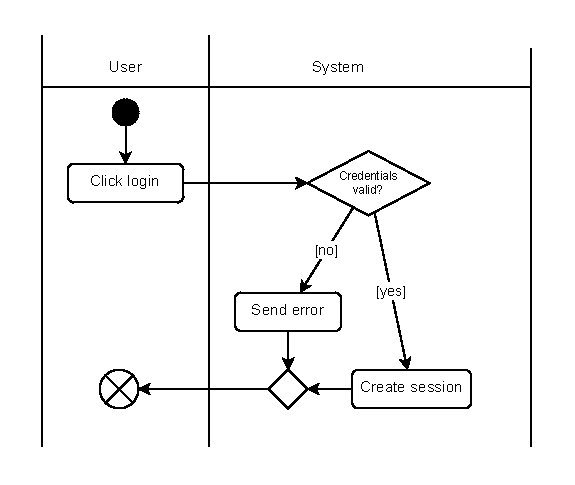
\includegraphics{ad-login}
    \caption{Activity diagram for the login flow.}
    \label{fig:ad:login}
\end{figure}

Figure~\ref{fig:ad:login} shows the steps that are required for the login process to finish.
The process ends either when the user has been logged in, and a session was created, or when the user failed to login.

\subsubsection{Signup}
\begin{figure}
    \centering
    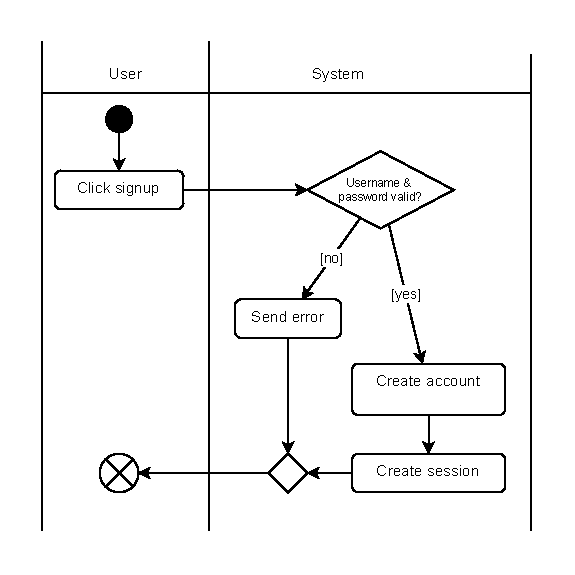
\includegraphics{ad-signup}
    \caption{Activity diagram for the signup flow.}
    \label{fig:ad:signup}
\end{figure}

Figure~\ref{fig:ad:signup} shows the steps that are required for the signup process to finish.
The process ends either when an account and session has been created, or when the user failed to signup.

\subsubsection{Select replic}
\begin{figure}
    \centering
    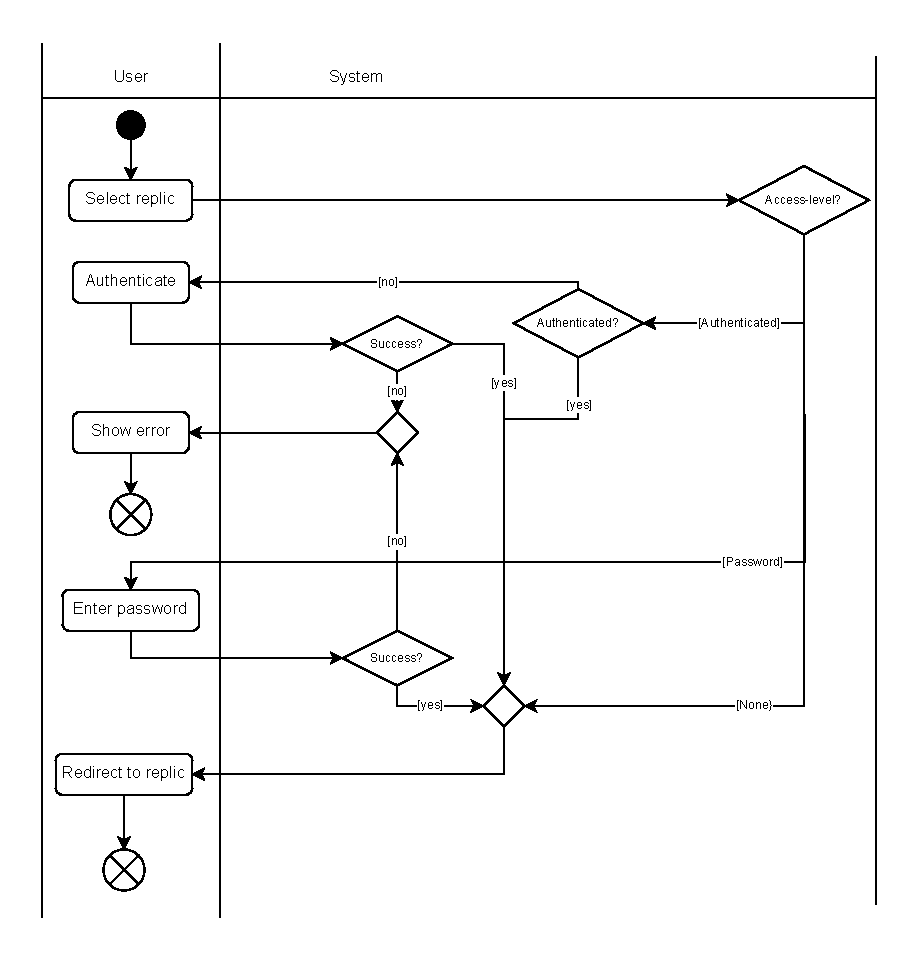
\includegraphics{ad-select-replic}
    \caption{Activity diagram for the select-replic flow.}
    \label{fig:ad:select-replic}
\end{figure}

Figure~\ref{fig:ad:select-replic} shows the steps to be done when the user selects a replic.
The flow finishes either when the user was redirected to the replic, or when the user could not be redirected.